%!TEX TS-program = xelatex
%!TEX encoding = UTF-8 Unicode

\documentclass[12pt]{extarticle}
% extarticle is like article but can handle 8pt, 9pt, 10pt, 11pt, 12pt, 14pt, 17pt, and 20pt text

\def \ititle {Origins of Mind}

\def \isubtitle {Lecture 08}

\def \iauthor {Stephen A. Butterfill}
\def \iemail{s.butterfill@warwick.ac.uk}
\date{}

%for strikethrough
\usepackage[normalem]{ulem}

\input{$HOME/Documents/submissions/preamble_steve_handout}

%\bibpunct{}{}{,}{s}{}{,}  %use superscript TICS style bib
%remove hanging indent for TICS style bib
%TODO doesnt work
\setlength{\bibhang}{0em}
%\setlength{\bibsep}{0.5em}


%itemize bullet should be dash
\renewcommand{\labelitemi}{$-$}

\begin{document}

\begin{multicols}{3}

\setlength\footnotesep{1em}


\bibliographystyle{newapa} %apalike

%\maketitle
%\tableofcontents




%---------------
%--- start paste


\def \ititle {Lecture 09}

\begin{center}

{\Large

\textbf{\ititle}

}



\iemail %

\end{center}






\section{Pointing: Reference and Context}

The \emph{block--slab} model of infant pointing \citep[compare][§2]{Wittgenstein:1953mm}:
(a) the activity occurs in a fixed context (e.g. buliding) and (b)
there is a fixed thing to be done in response to a point.

Comprehending pointing is not just a matter of locking onto the thing pointed to; it also
involves some sensitivity to context \citep[see][]{Liebal:2010lr}.

\subsection{Pointing: referent and context}

‘Already by age 14 months, then, infants interpret communication cooperatively, from a shared rather than an egocentric perspective’ \citep[p.\ 269]{Liebal:2010lr}.

‘The fact that infants rely on shared experience even to interpret others’ nonverbal pointing gestures suggests that this ability is not specific to language but rather reflects a more general social-cognitive, pragmatic understanding of human cooperative communication’ \citep[p.\ 270]{Liebal:2010lr}.



\section{A Puzzle about Pointing}

‘infant pointing is best understood---on many levels and in many ways---as depending on uniquely human skills and motivations for cooperation and shared intentionality, which enable such things as joint intentions and joint attention in truly collaborative interactions with others (Bratman, 1992; Searle, 1995).’
\citep[p.\ 706]{Tomasello:2007fi}

‘to understand pointing, the subject needs to understand more than the individual goal-directed behaviour. She needs to understand that by pointing towards a location, the other attempts to communicate to her where a desired object is located’
\citep[p.\ 6]{Moll:2007gu}.

\subsection{pointing vs linguistic communication}

‘the most fundamental aspects of language that make it such a uniquely powerful form
of human cognition and communication---joint attention, reference via perspectives,
reference to absent entities, cooperative motives to help and to share, and other
embodiments of shared intentionality---are already present in the humble act of infant
pointing.’ \citep[p.\ 719]{Tomasello:2007fi}

‘cooperative communication does not depend on language, […] language depends on it.’
\citep[p.\ 720]{Tomasello:2007fi}

‘Pointing may […] represent a key transition, both phylogenetically and
ontogenetically, from nonlinguistic to linguistic forms of human communication.’
\citep[p.\ 720]{Tomasello:2007fi}



\section{What is a communicative action?}

The confederate means something in pointing at the left box if she intends:

\begin{enumerate}

\item

that you open the left box;

\item

that you recognize that she intends (1), that you open the left box; and

\item

that your recognition that she intends (1) will be among your reasons for opening the left box.
\end{enumerate}

An inconsistent tetrad
\begin{enumerate}
\item 11- or 12-month-old infants produce and understand declarative pointing gestures.
\item Producing or understanding pointing gestures involves understanding communicative actions.
\item A communicative action is
  an action done with an intention to provide someone with evidence of an intention with the
  further intention of thereby fulfilling that intention.
\item Pointing facilitates the developmental emergence of sophisticated cognitive abilities
including mindreading
\end{enumerate}



\section{Syntax / Innateness}

Is the syntactic structure of ‘the red ball’ (a) flat or (b) hierachical?

\begin{center}

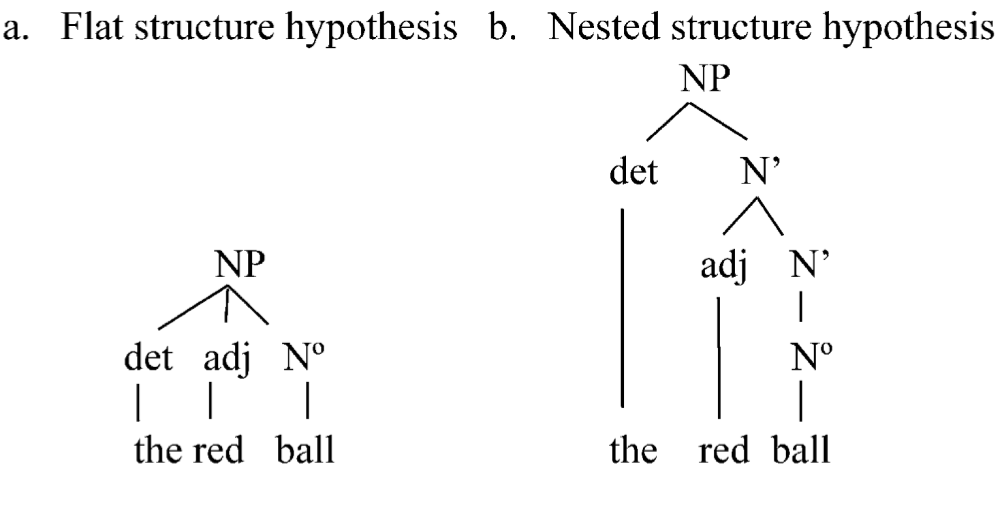
\includegraphics[scale=0.25]{../www.slides/src/raw/img/lidz_2003_fig0.neg.png}

\end{center}

\begin{center} from \citealp{lidz:2003_what} \end{center}

\begin{enumerate}



\item ‘red ball’ is a constituent on (b) but not on (a)


\item anaphoric pronouns can only refer to constituents



                \item In the sentence ‘I’ll play with this red ball and you can play with that one.’, the word ‘one’ is an anaphoric prononun that refers to ‘red ball’ (not just ball).
                \citep{lidz:2003_what,lidz:2004_reaffirming}.




\end{enumerate}

‘The assumption in the preferential looking task is that infants prefer to look at an image that matches the linguistic stimulus, if one is available’ \citep{lidz:2003_what}.

\subsection{Poverty of stimulus arguments}

How do poverty of stimulus arguments work? See \citet{pullum:2002_empirical}.

\begin{enumerate}

\item

Human infants acquire X.

\item

To acquire X by data-driven learning you'd need this  Crucial Evidence.

\item

But infants lack this Crucial Evidence for X.

\item

So human infants do not acquire X by data-driven learning.

\item

But all acquisition is either data-driven or innately-primed learning.

\item

So human infants acquire X by innately-primed learning .

\end{enumerate}

‘the APS [argument from the poverty of stimulus] still awaits even a single good supporting example’
\citep[p.\ 47]{pullum:2002_empirical}





%--- end paste
%---------------

\footnotesize
\bibliography{$HOME/endnote/phd_biblio}

\end{multicols}

\end{document}
